\documentclass[catalan,border=15pt,class=scrartcl,multi=minipage,parskip=half*]{standalone}

% encoding
\usepackage[utf8]{inputenc}
\usepackage[T1]{fontenc}
\usepackage{lmodern}
\usepackage{babel}

% formatting and fixes
\frenchspacing
\usepackage[style=spanish]{csquotes}
\MakeAutoQuote{«}{»}
\usepackage{bookmark}

% ADD ANY SPECIFIC PACKAGES HERE
% (CHEMISTRY, CODE, PUBLISHING)
\usepackage[usenames,dvipsnames,svgnames,table]{xcolor}
\usepackage{adjustbox}
\usepackage{booktabs}
\usepackage{mathtools}
\usepackage{commath}
\usepackage{tikz}
\usepackage{siunitx}
\usepackage{nicefrac}
\usetikzlibrary{calc}
\usetikzlibrary{arrows.meta}
\usetikzlibrary{automata}
\usepackage{minted}

% other options
\setcounter{tocdepth}{6}
\setcounter{secnumdepth}{2}

% hyperlink setup / metadata
\usepackage{hyperref}
\AfterPreamble{\hypersetup{
  pdfauthor={Xavier Mendez},
  pdfsubject={IPAV},
}}

% custom commands
\newcommand{\startpage}{\begin{minipage}{30em} \setlength{\parskip}{0.5em}}
\newcommand{\finishpage}{\end{minipage}}
\newcommand{\iopair}[2]{\( \left(#1\right) \rightarrow #2 \)}

\AfterPreamble{\hypersetup{
  pdftitle={Session 1. Basic operation of a spectrum analyzer based on the swept superheterodyne receiver principle},
}}

\begin{document}

\startpage
\paragraph{Activity	1.1.}

We set up the signal generator \& SA as requested. The marker verifies
the result we got in question 1.2.:

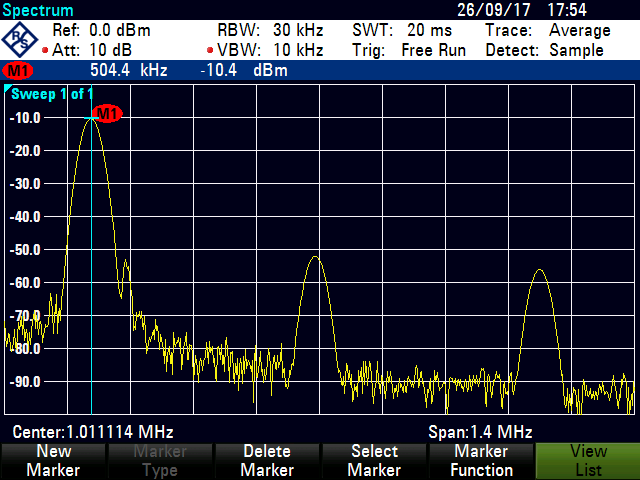
\includegraphics[width=\textwidth]{assets/1-1}

The SA produces higher order harmonics because the mixer that calculates the
product of the input and local oscillator signals isn't ideal and has some
amount of harmonic distortion.

\finishpage


\startpage
\paragraph{Activity 1.2.}

The annotations seen on the screen are:

\begin{description}
\item [Ref] The reference level, the highest decibel value shown in the screen.
It corresponds to the value at the top of the Y viewport axis.
\item [Att] The amount of attenuation applied to the input signal before the
mixer. More attenuation reduces the harmonic distortion but increases the noise
floor.
\item [RBW] The resolution bandwidth, the bandwidth of the IF bandpass filter.
\item [VBW] The video bandwidth, adjust the cutoff frequency of the smoothing
filter applied to the trace before being displayed (or averaged).
\item [SWT] The time it takes to do a full sweep to get a trace of the
frequencies shown at the viewport. This isn't directly modifiable, it's
calculated from the other parameters.
\item [Trig] The trigger mode, this determines when to start a swipe
(constantly, when an external signal indicates it, etc.).
\item [Trace] The operation applied to the trace, if any, just before
displaying (i.e. averaging with previous traces).
\item [Detect] The type of detector used to get the trace (sample the smoothened
signal, capture the maximum or minimum peaks, show the RMS, etc.).
\item [Center] The frequency that is displayed at the center of the X viewport
axis.
\item [Span] The length of the displayed frequency interval, from start to end
of the X viewport axis.
\end{description}

\finishpage


\startpage
\paragraph{Activity 1.3.}

We have adjusted the SA to show the wide shape around \SI{500}{\kilo\hertz}
when the resolution bandwidth is set to \SI{100}{\kilo\hertz}:

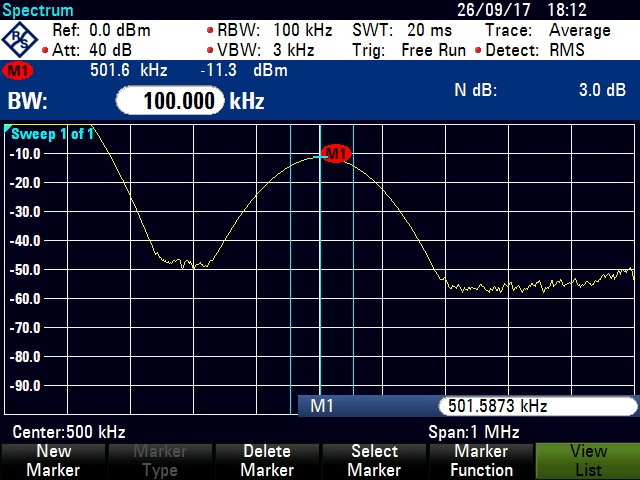
\includegraphics[width=\textwidth]{assets/1-3}

We can see how increasing the resolution bandwidth makes the shape wider.
In fact, we can see that the resolution bandwidth equals de \SI{-3}{\decibel}
bandwidth of the shape we see.

This matches our expectations, as what we're seeing is the actual delta
replaced by a sinc or similar shape (the impulse response of the bandpass
filter) whose bandwidth is controlled directly by the RBW.

\finishpage


\startpage
\paragraph{Activity 1.4.}

We have reconfigured the SA as requested:

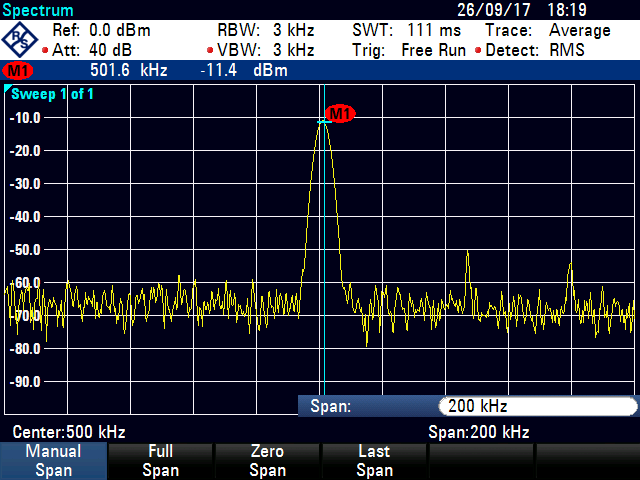
\includegraphics[width=\textwidth]{assets/1-4}

Then we enable zero span. This is what we see on screen:

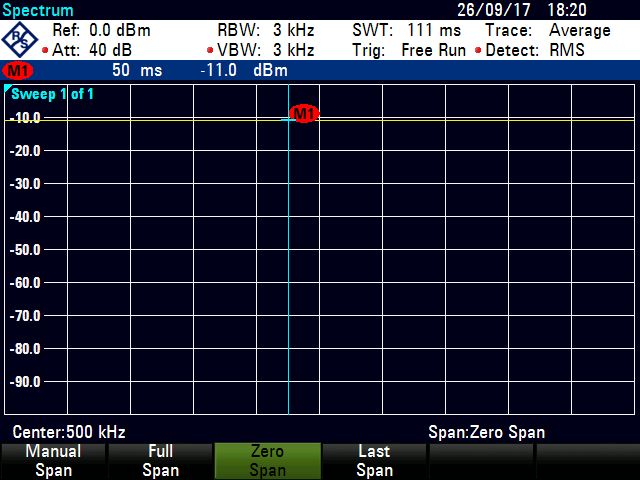
\includegraphics[width=\textwidth]{assets/1-4-2}

This trace represents the individual sample of the trace that was previously
at the center of the screen, i.e. the local oscillator is set to this fixed
frequency and no longer sweeps.

\finishpage


\startpage
\paragraph{Activity 1.5.}

We have reconfigured the SA as requested. The harmonics are now close to
the noise floor and this makes it difficult to measure their amplitude or
exact frequency:

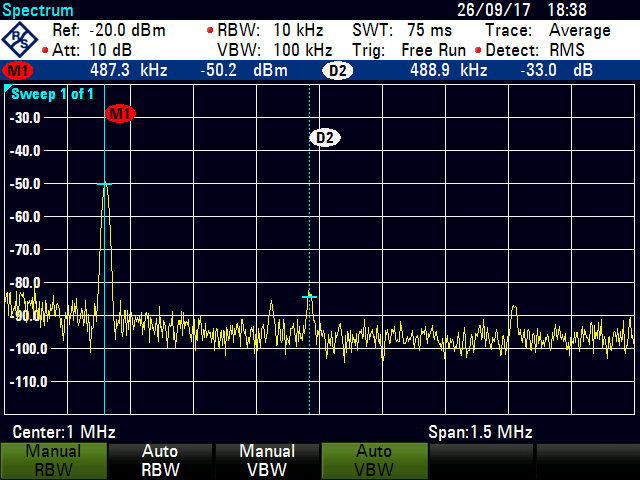
\includegraphics[width=\textwidth]{assets/1-5}

We have then reduced the video bandwidth to get a smoother trace:

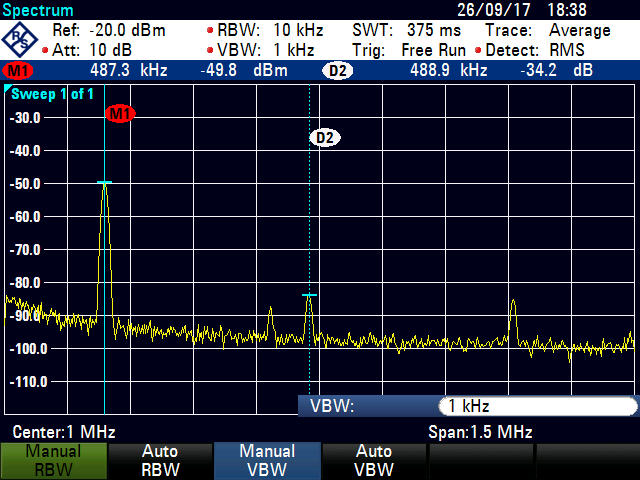
\includegraphics[width=\textwidth]{assets/1-5-2}

Finally, we have restored VBW to its previous value and enabled trace
averaging of the last 10 traces:

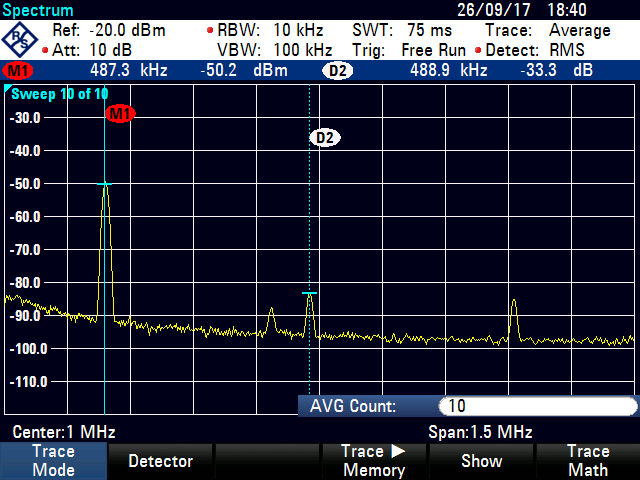
\includegraphics[width=\textwidth]{assets/1-5-3}

The first approach is \emph{spatial} smoothing; it may not be as effective and
it can increase the sweep time considerably, but changes in the spectrum are
still displayed quickly. The second uses \emph{temporal} smoothing; it gets
smoother traces but changes in the spectrum may display gradually or get
concealed.

\finishpage

\end{document}
